\documentclass[a4paper,11pt]{jsarticle}
\usepackage{ascmac}
\usepackage[dvipdfmx]{graphicx}
\usepackage{url}
% ######## measure #########
% # mm = 1mm = 2.85pt      #
% # cm = 10mm = 28.5pt     #
% # in = 25.4mm = 72.27pt  #
% # pt = 0.35mm = 1pt      #
% # em = width of [M]      #
% # ex = height of [x]     #
% # zw = width of [Kanji]  #
% # zh = height of [Kanji] #
% ##########################
% ##################### Portrait Setting #########################
% # TOP = 1inch + \voffset + \topmargin + \headheight + \headsep #
% #     = 1inch + 0pt + 4pt + 20pt + 18pt (default)              #
% # BOTTOM = \paperheight - TOP -\textheight                     #
% ################################################################
\setlength{\textheight}{\paperheight}   % 紙面縦幅を本文領域にする(BOTTOM=-TOP)
\setlength{\topmargin}{-10truemm}       % 上の余白を30mm(=1inch+4.6mm)に
\addtolength{\topmargin}{-\headheight}  % 
\addtolength{\topmargin}{-\headsep}     % ヘッダの分だけ本文領域を移動させる
\addtolength{\textheight}{0truemm}    % 下の余白も30mm(BOTTOM=-TOPだから+TOP+30mm)
% #################### Landscape Setting #######################
% # LEFT = 1inch + \hoffset + \oddsidemargin (\evensidemargin) #
% #      = 1inch + 0pt + 0pt                                   #
% # RIGHT = \paperwidth - LEFT - \textwidth                    #
% ##############################################################
\setlength{\textwidth}{\paperwidth}     % 紙面横幅を本文領域にする(RIGHT=-LEFT)
\setlength{\oddsidemargin}{-0.4truemm}  % 左の余白を25mm(=1inch-0.4mm)
\setlength{\evensidemargin}{-0.4truemm} % 
\addtolength{\textwidth}{-50truemm}     % 右の余白も25mm(RIGHT=-LEFT)

\title{課題3-1\\仕様書}

\author{清洲 星顕}
\date{更新日: 08/12}

\begin{document}
\maketitle
\section{はじめに}
\noindent
以下の機能を備えた簡易掲示板を作成する。\\
a.登録フォームを用意する。項目は名前とパスワード。\\
b.パスワードの入力確認をし、IDを生成する。IDとパスワードをユーザー情報としてデータベースに保存する\\
c.保存したユーザー情報を表示する

\section{フローチャート}
当掲示板のフローチャートを以下に図示する。
    \begin{figure}[htbp]
            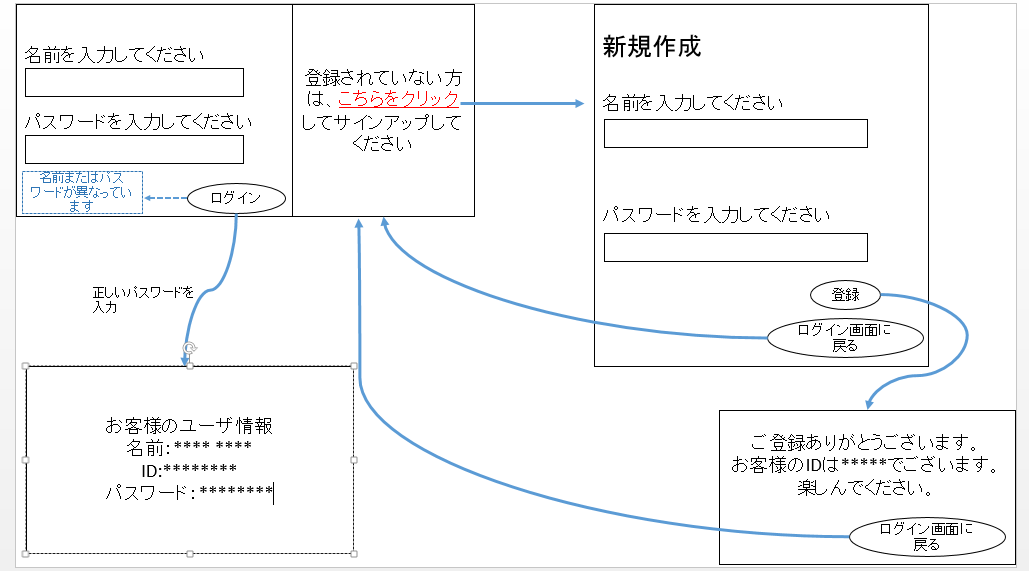
\includegraphics[clip,width=150mm]{intern_siyousho.PNG}
            \caption{フローチャート}
    \end{figure}
\newpage
\section{画面ごとの仕様}
\noindent


\subsection{ログイン画面(初めの画面)}
\noindent
名前とパスワードを入力してログイン認証を行う、すでに登録済みの場合はログイン完了後画面に遷移し、そうでない場合は、名前もしくはパスワードが異なっていることを伝える。\\
また、この画面では新規作成画面に遷移する画面を用意する。
    
\subsection{新規作成画面}
\noindent
名前とパスワードを入力して新規登録を行う。登録が終えるとIDが自動で生成され、ID、名前、パスワードをデータベースに保存する。登録が完了したら登録完了画面に遷移する。\\
新規作成を中断したいユーザのために"ログイン画面に戻る"ボタンを用意しておき、押すとログイン画面に遷移できるようにしておく。

\subsection{登録完了画面}
\noindent
IDをユーザに伝え、ログイン画面に遷移できるボタンを用意しておく。

\subsection{ログイン完了後画面}
\noindent
ユーザ情報を表示する。

\end{document}
